\documentclass[12pt,a4paper]{article}
\renewcommand{\baselinestretch}{1.5} 
\usepackage[toc,page]{appendix}
\usepackage[T1]{fontenc}
\usepackage[utf8]{inputenc}	
\usepackage[english]{babel}
\usepackage{graphicx}
% \usepackage[fontsize=14]{scrextend}
\usepackage{fancyhdr}
\usepackage{geometry}
\usepackage{varwidth}
\usepackage{chngpage}
\usepackage{array}
\usepackage{makecell}
\usepackage{float}
\usepackage{pdfpages}
\usepackage{svg}
\usepackage[noabbrev]{cleveref}
\usepackage[toc,page]{appendix}

% \usepackage[backend=bibtex,style=authoryear-icomp,sortlocale=de_DE,natbib=true,url=false, doi=true,eprint=false]{biblatex}
\usepackage{biblatex}
\bibliographystyle{ieeetr}
\bibliography{bibl.bib}

\pagestyle{fancy}
\fancyhf{}
% \title{Gaming Systems}
\title{Orchestration in the Internet of Things -\\ Towards a fully Integrated Solution}
\author{Jonas Burster - 20165136\\jburst16@student.aau.dk}


\date{xx.xx.2019}
\pagestyle{fancy}
\makeatletter
\let\runtitle\@title
\let\runauthor\@author
\makeatother
\lhead{\runtitle}
\rhead{Jonas Burster}

\graphicspath{{pictures/}}

\begin{document}
% \includepdf[pages=-]{PDF/page_0.pdf}
\maketitle

% \begin{figure}
% \vspace{-18cm}
%     \centering
%     \includegraphics[scale=0.4]{agillic-full-product-ball.png}
%     \label{fig:agillic-logo}
% \end{figure}
% \clearpage



\cfoot{\thepage}
\pagenumbering{Roman}

%\citetrackerfalse
\clearpage
\tableofcontents
% \listoffigures
\clearpage

\pagenumbering{arabic}
% \section{Glossary - either before report or after report -breaks reading flow!}
\section{Introduction - Frame it as a video IoT problem. IoT is nice but video in IoT is hard to manage especially live data. How to cope with a lot of real time data examplified in the leading video surveilance company.}
\subsection{Motivation - More reference; Less technical --> building better scalability and flexbility, modular vs monolithic, cloud --> Don't be so technical, more highlevel and grandual go into real challenges}
\subsection{Problem Definition}
\section{Methodology - Could also be in Introduction (if more than 1 page)}
\section{Motivate why Cloud is important to milestones --> Enabling surveilance in the cloud. Collecting data from video cameras and building flexible scaling service architecture around that, that can be extended upgraded to add functionalty and maintainability. Service Mesh is relevant for Milestone.}
\section{History of Microservice Architecture - integrate SOA from paper - lose coupling!!! using descriptive messages rather de; microservice came from SOA; Network function virtualization and software defined network (only look at it)}
\section{State of the Art (Competitor analysis)}
\section{Literature Review/ What is a Service Mesh --> merge with history}

\section{Requirements from Milestone}
\subsection{Interviews (Head of Research and Cloud Orchestration Lead + With Professional from Istio Gathering in Cph)} 
\subsection{Functional Requirements ; Each Req should have source and reason}
\subsection{Non-Functional Requirements; source and reason}
\subsection{MoSCoW --> Give reason for prioritize certain feature (discuss what I can do and lower priority could be part for future.}
\section{Istio}
\subsection{Capabilities - Consider removing this. }
\subsection{Testing Istio Overhead in a Generic Setup}

\section{Implementation in Milestone}
\subsection{The current C2C? setup at Milestone}
\subsection{Platform Improvements from Istio}
\subsection{Chaos Testing}
\subsection{Benchmarking before vs after}
\section{Reflection/ Evaluation}
\section{Future Work}
\section{Conclusion}





% \section{Glossary}

- explain the major technologies and concepts\\
- Keep simple and short ( use same reference style for outside\\ literature)\\
- 

\subsection{Internet of Things}
The Internet of Things (IoT) describes 

\subsection{Fog Computing}
Fog computing describes the architectural style of carrying out computation, storage and communication (locally) at the edge of the network \citep{fogComputing:def}. It thus brings with it a whole new set of problems and challenges compared to the cloud. According to \citep{Introducing:kubeedge}, a senior software engineer in the field cloud messaging and IoT platforms at Red Hat, its three main advantages over the cloud are: "Low latency, availability and locality". 

\subsubsection{OSI Model}
Similarly to the Kubernetes and Istio documentation this report will use the 7-Layer OSI model \cite{IstioLayers61:online}


\subsection{CI/CD}
CI/CD is an automated approach to software development. CI stands for continuous integration and means continuously merging working code with the master branch, while testing for code quality via unit and integration tests \citep{shahin2017continuous}. CD stands for continuous development (sometimes also deployment) and means running 
\section{Introduction}
\begin{displayquote}
\textit{\textbf{\Huge{``}}
\large{Around 10\% of enterprise-generated data is created and processed outside a traditional centralized data center or cloud. By 2025, Gartner predicts this figure will reach 75\%.\cite{gartnerEdgeComputing:online}}
\textbf{\Huge{''}}}
\\[1pt]
\raggedleft{{\rm --- Gartner}}
\end{displayquote}
Data has never been as ubiquitous as it is today. Not only do our mobile phones constantly generate data but also the things we wear, use and own are now generating data. Not only the private sector is effected by this data revolution also the industry is embracing new technologies to gather data to automate processes. Some factories are even operated entirely self-sufficient without any human intervention. These factories are called "lights-out factories" and are becoming more and more popular\cite{wheresmyRobotLightsOut33:online}. In a world where data is everywhere the computing power to process this data has to be everywhere as well. Relying solemnly on centralized servers will eventually topple the system. The estimate by Gartner that 75\% of data will be generated and processed outside traditional data centers clearly shows decentralized architectures are here to stay.\\
In a curated report from the economist in 2015 the authors conclude that "cloud computing has the potential to disrupt entire industries, reshape businesses and markets and change the way we think about information"\cite{PuttogetEconomistCloud13:online}. Much of this success can be attributed to Kubernetes. It is a platform for container orchestration and was donated by Google to the open source community in 2014\cite{WhatisKubernetes87:online}. It enables the abstraction of hardware from deployments and provides much of the simplicity of Platform as a Service (Paas).\\
Edge computing is the term used for processing and storing data on the edge of the network. Fog computing is a subform of edge computing where the edge part is tightly integrated with the cloud to enhance both systems. This brings new possibilities and challenges to system designers.\\
In this thesis I will also construct an exemplary fog setup to remotely monitor and control lights to see the areas Kubernetes excels in but also it shortcomings. Finally, I will argue that Kubernetes should be the default platform for both cloud and edge computing to provide a homogeneous system for easy development, management and monitoring. Kubernetes is not fully optimized for this task yet, but the sooner it is the better for the entire industry.



% \comment{
In 2015, the Cloud Native Computing Foundry (CNCF) was founded under the 
umbrella organization of the Linux Foundation. 

https://blogs.gartner.com/thomas_bittman/2017/03/06/the-edge-will-eat-the-cloud/

Since edge devices can also produce terabytes of data, taking the analytics closer to the source of the data on the edge can be more cost-effective by analyzing data near the source and only sending small batches of condensed information back to the centralized systems.
}
\subsection{Motivation}
Edge computing, and especially fog computing, are emerging as a new paradigm on how to structure the computational resources of a system. It enables technology to operate very close to the user or thing and places no additional burden on the core network or servers. According to Dejan Bosanac, a senior software engineer at Red Hat in the field of cloud messaging and IoT platforms, these devices have three main advantages over the cloud due to their proximity to the devices and end users: 
\begin{displayquote}
{\textbf{``Low latency, availability and locality''}}\cite{IntroducingDejanBosanac:KubernetesIoTEdgeWorkingGroup}
\end{displayquote} 
Edge computing is set to have profound changes on mobile computing and Industrial IoT (IIoT) and has been described as "enabler for the Industrial Internet of Things"\cite{steiner2016fogenablerIIoT} in the academic literature.

However, there is no industry wide standard for structuring or deploying edge resources. No software has yet emerged and taken the industry by storm and became the de-facto standard. Kubernetes has done so in the cloud and I am going to argue Kubernetes will be the technology to transform the edge from an isolated into an active part in the data processing pipeline. Importantly, Kubernetes not only has the advantage of fog computing, i.e. cloud aware edge device or enabling offline edge clusters, but also includes central and standardized monitoring and networking. As most systems will be connected to the Internet one way or another in the future, fog computing stands to be the primary use case, but it is not required.

For edge computing security, hardware restrictions, isolation, fault tolerance and more are immensely important issues and Kubernetes already has the tools and features to solve many of these problems. Importantly, Kubernetes allows for remote controlling and monitoring of systems and works actively to ensure the desired state of the cluster.

\comment{


In this thesis I will thus explore how Kubernetes can facilitate fog computing and what challenges still have to be solved.
}
\subsection{Problem Area}\label{sec:problemArea}
\comment{
Why are IoT Gateways so hard to get right? Why is the edge so hard to get right?
 - Diversity
 - Security
 - Stability
}
% Main text
{
Mobile devices profoundly changed the way computers interact with each other. When these devices became a commodity in the 90s\footnote{Back then smartphones were called personal digital assistant (PDA).}, the way we manage computing power needed to change to accommodate intensive tasks on light weight computers. Researchers started to experiment with local, remote (cloud) and mixed execution also called adaptive cloud offload. The researchers found huge gains from adaptive cloud offloading with a high enough bandwidth and concluded "the convergence of mobile computing and cloud computing enables new multimedia applications that are both resource-intensive and interaction-intensive."\cite{noble1997agileIoTGatewayOdyssey}. As one of the researches later put it "while mobile elements will undoubtedly improve in absolute ability, they will always be at a relative disadvantage."\cite{satyanarayanan2015briefHistoryIoTGateway}\\
Today, we not only have smartphones, which have gotten quite powerful, but tiny IoT devices which are often build to last months on a single battery and have very, very limited processing power. New architectural patterns and communication technologies emerged to support these ultra low power and processing requirements. This lead to a fractured landscape where many manufacturers developed their own technology, mostly as closed source. There were some open source efforts but none taking over the entire industry. It was not felt necessary to have a centralized control plane, where updates could be scheduled and the system monitored. Applications did not have any isolation from the host operating system and often times security updates were not even deemed necessary, which left many IoT gateways and devices vulnerable to attacks leading to serious attacks like the Mirai botnet\cite{7971869MiraiAndOtherBotnetLinux}. Its important to note, that most attacks target Linux devices and not microcontrollers running on real time operating systems (RTOS).\\
In 2009, the National Science Foundation rejected a paper because \textit{``Many panelists do not agree with the premise of the proposal in which distant cloud computing incurs too high latency to be acceptable by mobile applications. They question the validity of such assumption as the proposal provides no real data to justify it[...]''}\cite{satyanarayanan2015briefHistoryIoTGateway}. Much has changed since then. The smartphone revolution greatly increased the data produced by mobile devices and the need for speed, security and privacy. Researches did not foresee the explosion in IoT and the onset of a new wave of data producers bundled under the term Indutrial IoT (IIoT). It includes hundreds and thousands of IoT devices working together in factories, logistic warehouses, connected vehicles (CV), smart grid etc. In 2012 a widely cited paper "Fog Computing and Its Role in the Internet of Things"\cite{fogComputing:def} was published, establishing the need for IoT gateways connected to the cloud. It concluded that the amount and high frequency of produced data is too much for the cloud and pre-processing on the edge is needed for both latency and efficiency.\\
However, establishing the need for edge computing is not the same as solving it. Since then many papers have been published with titles such as "The Internet of Things Has a Gateway Problem"\cite{zachariah2015internetOfThingsHasGatewayProblem}. At the same time, researchers used custom IoT gateway solutions and achieved impressive results. In one experiment, they achieved over 80\% performance increase in certain scenarios rightly titling their paper "From Cloud Computing to Fog Computing: Unleash the Power of Edge and End Devices"\cite{hong2017fromCloudtoIoTGatewayUnleashingTHePower}.\\
}

\subsubsection{Expected Outcome}
This thesis will implement a fog system with Kubernetes at its core. It will explain how Kubernetes can aid in many challenges facing the edge and give insights into Kubernetes resources important for the edge, including containers, and the best practices. Such a system could become the industry norm influencing millions of deployments in many diverse industries. It would improve communication and observability and finally put a halt to most malicious attacks by reducing the attack surface to a bare minimum.\\

\subsubsection{Research Question}
In essence, the research question for this thesis is:
\begin{displayquote}\begin{center}
{\textit{\textbf{How can Kubernetes facilitate edge computing, what challenges does it solve and where are its shortcomings?}}}
\end{center}\end{displayquote}

\subsubsection{Delimitation} \label{sec:delimitation}
\comment{
Exclude non Kubernetes related technologies.\\
Exclude mobile devices.\\ All a lot of technologies are still relevant but not discussed. In future work mention it
Exclude hardware.\\
Exclude Sort of 5g and advances in mobile technologies.\\ Rich field
Exlude infrastructure edge.\\
Exclude RTOS.\\
}








\comment{


Edge computing started as a way to give mobile devices more power.
Technopedia defines a mobile device as a "handheld tablet or other device that is made for portability, and is therefore both compact and lightweight"\cite{WhatisaM95TechnopediaMobileDevice:online}, it includes laptops, smartphones, tables etc.  As Mahadev Satyanarayanan put it "while mobile elements will undoubtedly improve in absolute ability, they will always be at a relative disadvantage."\cite{satyanarayanan2015briefHistoryIoTGateway} Back then, researchers experimented with local, remote (cloud) and mixed execution also called adaptive
cloud offload. Assessing the three variants for voice recognition, video playback and web browsing locally, the researchers found huge gains from adaptive cloud offloading with a high enough bandwidth and concluded "the convergence of mobile computing and cloud computing enables new multimedia applications that are both resource-intensive and interaction-intensive."\cite{noble1997agileIoTGatewayOdyssey}. This lead to an explosion in cloud development. The Internet started out with a decentralized servers around the world. But over the years technologies were invented for orchestration across these distant servers, but also isolation for the local deployments. Probably the two main technological standards evolving where containers with containerd and orchestration with Kubernetes. \\
Traditionally, mobile devices connected to a gateway, which was mainly a router operating at L3\footnote{L3 stands for Layer 3, the networking layer in the OSI model.} to route packets and translate between different types of network protocols. \cite{lee2017futureOfIoT}. However, according to Dejan Bosanac, a senior software engineer at Red Hat in the field of cloud messaging and IoT platforms, due to their proximity to the sensors and the end user, these devices have three main advantages over the cloud: 
\begin{displayquote}
{\textbf{``Low latency, availability and locality''}}\cite{IntroducingDejanBosanac:KubernetesIoTEdgeWorkingGroup} - Dejan Bosanac.
\end{displayquote}
Because of these advantage researchers construct hybrid systems, in which devices operating on the edge of the network play an active role in the data processing pipeline. This architectural style of carrying out substantial amount of computation and storage at the edge is called "edge computing" \cite{fogComputing:def}. \Cref{fig:iotDeviceSetup} shows where the gateway is positioned in the current communication setup. 
 \begin{figure}[!h]
     \centering
     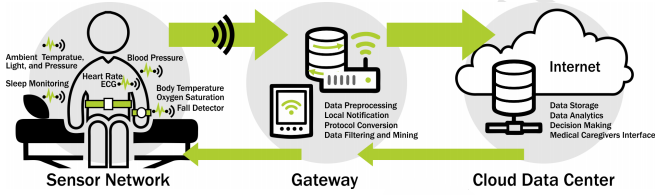
\includegraphics[scale=2]{figures/iotSetup.png}
     \caption{The position of the gateway in the current Internet infrastructure\cite{iotGatewaySlavesGraph}.}
     \label{fig:iotDeviceSetup}
 \end{figure}\\
But not everyone in the academic world was convinced that edge computing was indeed the way forward. 
However, establishing the need for edge computing is not the same as solving all problems though, and since then many papers have been published with titles such as "The Internet of Things Has a Gateway Problem"\cite{zachariah2015internetOfThingsHasGatewayProblem}. At the same time, researchers used custom IoT gateway solutions in their research and achieved impressive results. In one experiment, they achieved over 80\% performance increase in certain scenarios rightly titling their paper "From Cloud Computing to Fog Computing: Unleash the Power of Edge and End Devices"\cite{hong2017fromCloudtoIoTGatewayUnleashingTHePower}. Adding further to the problem of standardization is that IoT, especially IIoT, and mobile device have very different requirements.\\
This is the current place of the industry. There is a common agreement that fog computing is essential in the future, but no standard and open solution was developed yet. There is considerable effort in the academic world and in the industry to establish such a standard, one such initiatives is the Kubernetes IoT Edge working group under the Cloud Native Computing Foundry (CNCF). 




The space between the cloud and IoT and mobile devices, can be confusing at times. Knowing the history of IoT and the cloud is vital to understand the current developments. This, the methodology and the delimitation of this thesis will be discussed in the reminder of this section.\\




The terms used in the academic world and the industry are often different and many concepts partially overlap and complement each other making it hard to clearly categorize solutions. This is mainly due to ever evolving hard- and software, changing the possibilities of the devices and the entire landscape. It is thus imperative to clearly outline the key terms and design philosophies used of this thesis as well as presenting already existing solutions and how they compare to each other. These aspects are part of \cref{sec:eSOTA}, \nameref{sec:eSOTA}.\\
\Cref{sec:analysis}, \nameref{sec:analysis}, will lay the foundation to the actual implementation. We will motivate our design choices with academic and industry literature as well as with interviews from industry leaders. The focus of this thesis will be on the software and the requirements of the software to define and use the edge. Ultimately, it does not matter whether increases in performance and security come from better hardware or software, as long as the requirements are met. Consequently, the requirements will be ordered via the MoSCoW method. I will analyze the existing protocols, mainly for the application layer, and the data serialization method. Kubernetes is at the heart of this thesis implementation and extra sections will discuss what tricks Kubernetes already offers to control an edge cluster from the cloud and what might be missing. Additionally, I will look at extensions Kubernetes offers and how they could be useful in an IoT environemnt.\\


}

\comment{
The main focus is going to be on the software driving fog computing with an emphasize on IoT device and less mobile devices. 
We use a three tier layered network topology shown in \cref{fig:networkTopology3Layer}.
\begin{figure}[h!]
    \centering
    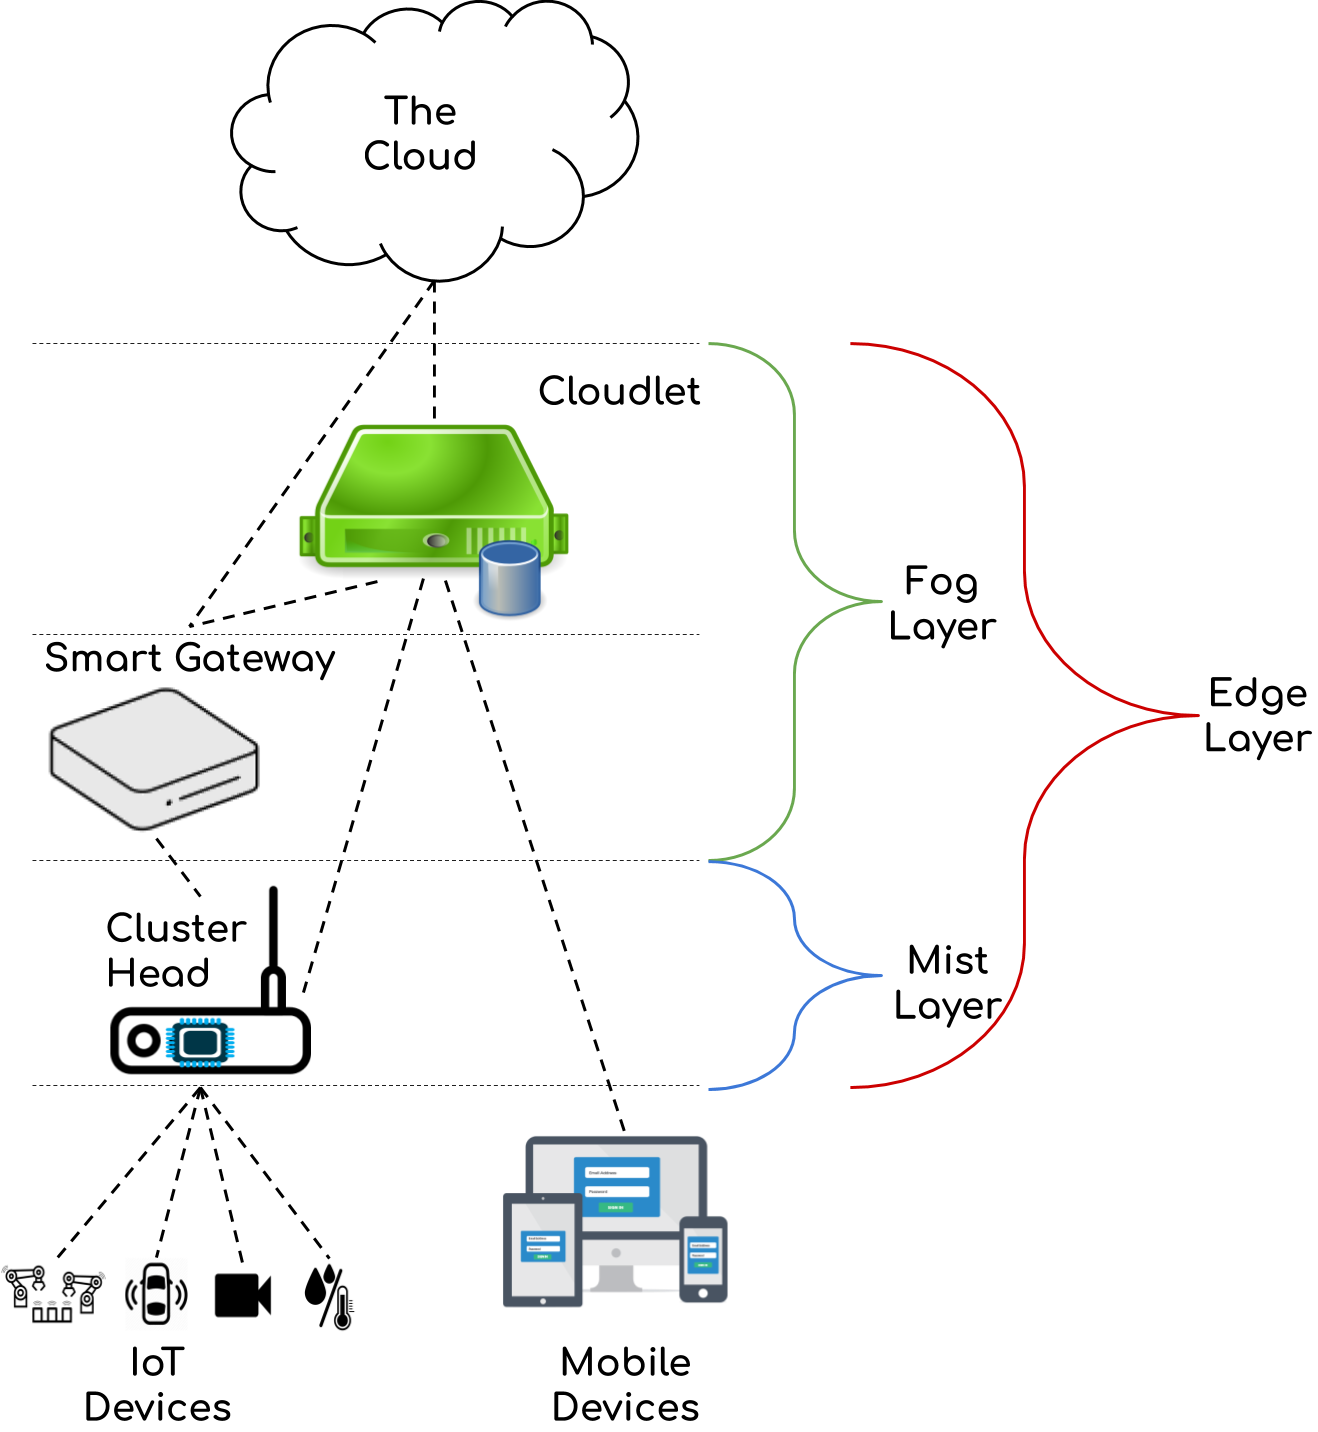
\includegraphics[scale=0.15]{figures/network-topology-3-layer.png}
    \caption{Three tier layer network topology, similar to \cite{nsa2017theNextWaveIoTDefinitions}}
    \label{fig:networkTopology3Layer}
\end{figure}
% Describe figure:
The cloud layer is made up of the 

% More detail
The cloud is the one layer where the authors think the technology stack is set. We expect Linux and Kubernetes, the de-facto standard for cloud orchestration, to be here to stay for the foreseeable future. This implies the same for x86\_64 and ARM, the only CPU architectures being supported by Linux. The Internets communication will remain in IPv4 and increasingly IPv6 for the Internet layer and TCP and UDP for the transport layer.\\ 
Quite the contrary is true for the bottom layer, IoT devices and mobile devices, although for the latter to a lesser extend. Communication in the IoT space is very diverse. Some protocols like 802.11 and Mobile

We expect IoT devices to have different software and different 
This can, but must not, include a control plane
The aim is to find the most promesing solution and 




Promesing solution with deep integration into K8s.


In essence, fog is the standard, and edge is the concept. Fog enables repeatable structure in the edge computing concept, so enterprises can push compute out of centralized systems or clouds for better and more scalable performance.
https://www.cisco.com/c/en/us/solutions/enterprise-networks/edge-computing.html


As it's name implies its aim is to develop an edge solution with Kubernetes support.

The need for smart IoT Gateways or fog computing is well established. They make it possible to 

Their design however is not. 
While the problems at the IoT edge — connectivity, manageability, scalability, reliability, security — are being solved as point solutions by enterprises and ecosystem players, there is a need for a foundational industry-wide standard for managing distributed IoT workloads.





IoT has seen a rapid growth over the last few years. According to IoT Analytics the total number of IoT devices is set to surpass the total number of other connected devices around 2021 \cite{StateofIoT:online}. Further, most IoT devices will be used in WPAN \footnote{Wireless Private Area Networks includes technologies like Zigbee,Z-wave and Bluteooth} and WLAN\footnote{Wireless Local Area Networks includes mainly Wi-Fi}. 
% In contrast to 5G, these technologies don't connect to an access point from an Internet provider but rather require another user operated device to connect to the Internet, a so called "gateway"


But fog computing does not come without its drawbacks. Depending on the protocol edge devices need to be close to their peers and slaves and physically accessible for maintenance. Which also poses a major security risk as they could be accessed by malicious intruders. The software maintenance is another critical aspects. Often IoT and edge devices are not update and patched with critical consequences. The "2016 Dyn cyberattack" used IoT devices like residential gateways, smart fridges, baby phones ect. to bring down the DNS-Servers operated by Dyn making large part of the Internet unaccessible for hours\cite{dynAttack}. The authors also stress that "large number of IoT devices are accessible over public Internet" and that "security (if considered at all) is often an afterthought in the architecture of many wide spread IoT devices"\cite{dynAttack}.\\
The question is then, how can manage and secure those devices. In this thesis, I will solely be concerned with the software aspect, which can mitigate some effects of exposing physical hardware to more accessible places.\\
Many challenges facing edge devices today have already been solved, although in a slight different context: The cloud\cite{IntroducingDejanBosanac:KubernetesIoTEdgeWorkingGroup}. In the cloud 




% Note: Maybe make a graph cloud setup, user connecting to nodes, VS fog computing, sensors and users connecting to gateways and gateway to cloud.  https://www.einfochips.com/blog/iot-gateways-drivers-for-fog-computing/

Kubernetes IoT Edge Working Group is a collaboration between Eclipse IoT Working Group and its 40-member companies, 35 open source projects, and Kubernetes ecosystem. It will define terminology, identify gaps in deployment and management, and educate the market on common use cases.
https://www.dailyhostnews.com/eclipse-foundation-and-cncf-working-together-to-bring-kubernetes-to-iot-edge
}
% \subsubsection{A Brief History}
\comment{
Why are IoT gateways important?
How did it come to be?
How did it start?
Why is it now, that many companies have interest?
}
Mobile devices profoundly changed the way computers interact with each other. Technopedia defines a mobile device as a "handheld tablet or other device that is made for portability, and is therefore both compact and lightweight"\cite{WhatisaM95TechnopediaMobileDevice:online}, it includes laptops, smartphones, tables etc. When these devices became a commodity in the 90s\footnote{Back then smartphones were called personal digital assistant (PDA).}, the way we manage computing power needed to change to accommodate intensive tasks on light weight computers. As Mahadev Satyanarayanan put it "while mobile elements will undoubtedly improve in absolute ability, they will always be at a relative disadvantage."\cite{satyanarayanan2015briefHistoryIoTGateway} Back then, researchers experimented with local, remote (cloud) and mixed execution also called adaptive
cloud offload. Assessing the three variants for voice recognition, video playback and web browsing locally, the researchers found huge gains from adaptive cloud offloading with a high enough bandwidth and concluded "the convergence of mobile computing and cloud computing enables new multimedia applications that are both resource-intensive and interaction-intensive."\cite{noble1997agileIoTGatewayOdyssey}. This lead to an explosion in cloud development. The Internet started out with a decentralized servers around the world. But over the years technologies were invented for orchestration across these distant servers, but also isolation for the local deployments. Probably the two main technological standards evolving where containers with containerd and orchestration with Kubernetes. \\
Traditionally, mobile devices connected to a gateway, which was mainly a router operating at L3\footnote{L3 stands for Layer 3, the networking layer in the OSI model.} to route packets and translate between different types of network protocols. \cite{lee2017futureOfIoT}. However, according to Dejan Bosanac, a senior software engineer at Red Hat in the field of cloud messaging and IoT platforms, due to their proximity to the sensors and the end user, these devices have three main advantages over the cloud: 
\begin{displayquote}
{\textbf{``Low latency, availability and locality''}}\cite{IntroducingDejanBosanac:KubernetesIoTEdgeWorkingGroup} - Dejan Bosanac.
\end{displayquote}
Because of these advantage researchers construct hybrid systems, in which devices operating on the edge of the network play an active role in the data processing pipeline. This architectural style of carrying out substantial amount of computation and storage at the edge is called "edge computing" \cite{fogComputing:def}. \Cref{fig:iotDeviceSetup} shows where the gateway is positioned in the current communication setup. 
 \begin{figure}[!h]
     \centering
     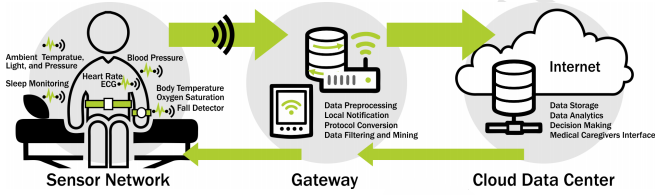
\includegraphics[scale=1.8]{figures/iotSetup.png}
     \caption{The position of the gateway in the current Internet infrastructure\cite{iotGatewaySlavesGraph}.}
     \label{fig:iotDeviceSetup}
 \end{figure}\\
But not everyone in the academic world was convinced that edge computing was indeed the way forward. In 2009, the National Science Foundation rejected a paper because \textit{``Many panelists do not agree with the premise of the proposal in which distant cloud computing incurs too high latency to be acceptable by mobile applications. They question the validity of such assumption as the proposal provides no real data to justify it[...]''}\cite{satyanarayanan2015briefHistoryIoTGateway}. Much has changed since then. The smartphone revolution (do I need to cite this? Is it a term I can actually use?) greatly increased the data produced by mobile devices and the need for speed and privacy. Researches did not foresee the explosion in IoT and the onset of a new wave data producers bundled under the term Indutrial IoT (IIoT). It includes hundreds and thousands of IoT devices working together, for example in factories, logistic warehouses, connected vehicles (CV), smart grid etc. In 2012 a widely cited paper "Fog Computing and Its Role in the Internet of Things"\cite{fogComputing:def} was published, establishing the need for IoT gateways connected to the cloud. The amount and high frequency of produced data is just too much to only handle in the cloud. Pre-processing on the edge is needed for both latency and efficiency.\\
However, establishing the need for edge computing is not the same as solving all problems though, and since then many papers have been published with titles such as "The Internet of Things Has a Gateway Problem"\cite{zachariah2015internetOfThingsHasGatewayProblem}. At the same time, researchers used custom IoT gateway solutions in their research and achieved impressive results. In one experiment, they achieved over 80\% performance increase in certain scenarios rightly titling their paper "From Cloud Computing to Fog Computing: Unleash the Power of Edge and End Devices"\cite{hong2017fromCloudtoIoTGatewayUnleashingTHePower}. Adding further to the problem of standardization is that IoT, especially IIoT, and mobile device have very different requirements.\\
This is the current place of the industry. There is a common agreement that fog computing is essential in the future, but no standard and open solution was developed yet. There is considerable effort in the academic world and in the industry to establish such a standard, one such initiatives is the Kubernetes IoT Edge working group under the Cloud Native Computing Foundry (CNCF). 


% \Cref{sec:problemArea}, \nameref{sec:problemArea}, will explain what challenges system designers face on the edge and why developing a standard is so hard.



























\subsection{Methodology}
The methodology describes the theoretical background for the methods applied in this thesis and ensures consistency across related work in the field.
The section Extended State of the Art is meant to provide the reader with an objective and complete overview of the research area. Following, in the Analysis section use cases are used to gather requirements. These are then prioritized according to the importance and feasibility for the desired system. Finally, in the Implementation, the system based on these requirements is implemented following a software development method and the priorities of the requirements.\\[5mm]
\textbf{\leftskip25mm\textit{Existing Solutions}}\\
The existing solutions section gives an objective presentations of already existing solutions in the field and sheds a light on how widely adopted systems or new once solve particular problems. It is not about the product but rather what the product tries to achieve and how.\\[5mm]
\textbf{\leftskip25mm\textit{Use Cases}}\\
Use cases are a way to find requirements\cite{UseCase94Fowler:online}. They can appear in the form of UML diagrams or written text. In this thesis only the written text version is used as the UML diagrams "[...]are of little value" and "the key value of use cases lies in the text" according to Martin Fowler\cite{UseCase94Fowler:online}. As the developed system is only a prototype I will use the "casual template for low-ceremony projects" from the book "Writing Effective Use Cases" from Alistair Cockburn\cite{cockburn2000writingUseCases}.\\[5mm]
\textbf{\leftskip25mm\textit{Functional Requirements}}\\
Functional Requirements state what services a system should provide, how it reacts to particular inputs, and how it should behave under particular circumstances\cite{sommerville2011software}. They are derived from the use cases and the state of the art and are the foundation for the implementation.\\[5mm]
\textbf{\leftskip25mm\textit{MoSCoW}}\\
The MoSCoW method is a way to structure the requirements according to the needs of the stakeholders involved\cite{sommerville2011software}. It is an acronym for "Must, Should, Could, Would". It helps to plan time and resources in a project so that the requirements with a higher ranking are finished first.\\[5mm]
\textbf{\leftskip25mm\textit{Agile Software Development Method}}\\
The software development method is a way to structure the development of software. An agile method emphasize development cycles to increase the transparency and flexibility during the software development. It decreases the risk of failure by constantly reevaluating the product. The agile manifest developed by industry experts\cite{beck2001manifestoAgile} has four main values: Individuals and Interactions over processes and tools; Working Software over comprehensive documentation; Customer Collaboration over contract negotiation; Responding to Change over following a plan. These are the foundation for a working agile software development method.

% \subsubsection{Delimitation} \label{sec:delimitation}
\comment{
Exclude hybrid cloud\\
Exclude non Kubernetes related technologies.\\
Exclude mobile devices.\\
Exclude hardware.\\
Exclude Sort of 5g and advances in mobile technologies.\\
Exlude infrastructure edge.\\
Exclude multi-cluster\\

}

\section{Extended State of the Art}\label{sec:eSOTA}

\begin{displayquote}
\textit{\textbf{\Huge{``}}}
\textit{\large{
Kubernetes has massive potential for handling IoT workloads on the edge by providing a common control plane across hybrid cloud and edge environments to simplify management and operations\cite{ioFogMainBlog:online}.
}}
\textit{\textbf{\Huge{''}}}
\\[1pt]
\raggedleft{{\rm --- Mike Milinkovich, CEO of Eclipse Foundation}}
\end{displayquote}

\comment{
https://www.iaria.org/conferences2016/filesICSNC16/Softnet2016_Tutorial_Fog-MEC-Cloudlets-E.Borcoci-v1.1.pdf

this paper has it nailed down with terms https://arxiv.org/pdf/1812.00591.pdf 
}

\subsection{Terms and Definitions} \label{sec:definitions}
The IoT and edge landscape is hard to understand, especially because terms are loosely and inconsistently defined. Similar is true for the cloud but it uses less diverse technologies and is thus less confusing. This section will explain the network topology, key terms and their concepts as the foundation for the following report.\\
\vspace{0.5mm} \ \\
\textbf{\textit{Network Topology}}\\
\Cref{fig:networkTopology3Layer} shows the network topology used in this report. 
% The focus will be on the management and security of the device edge as well as its interaction with the IoT devices themselves. 
\begin{figure}[H]
    \centering
    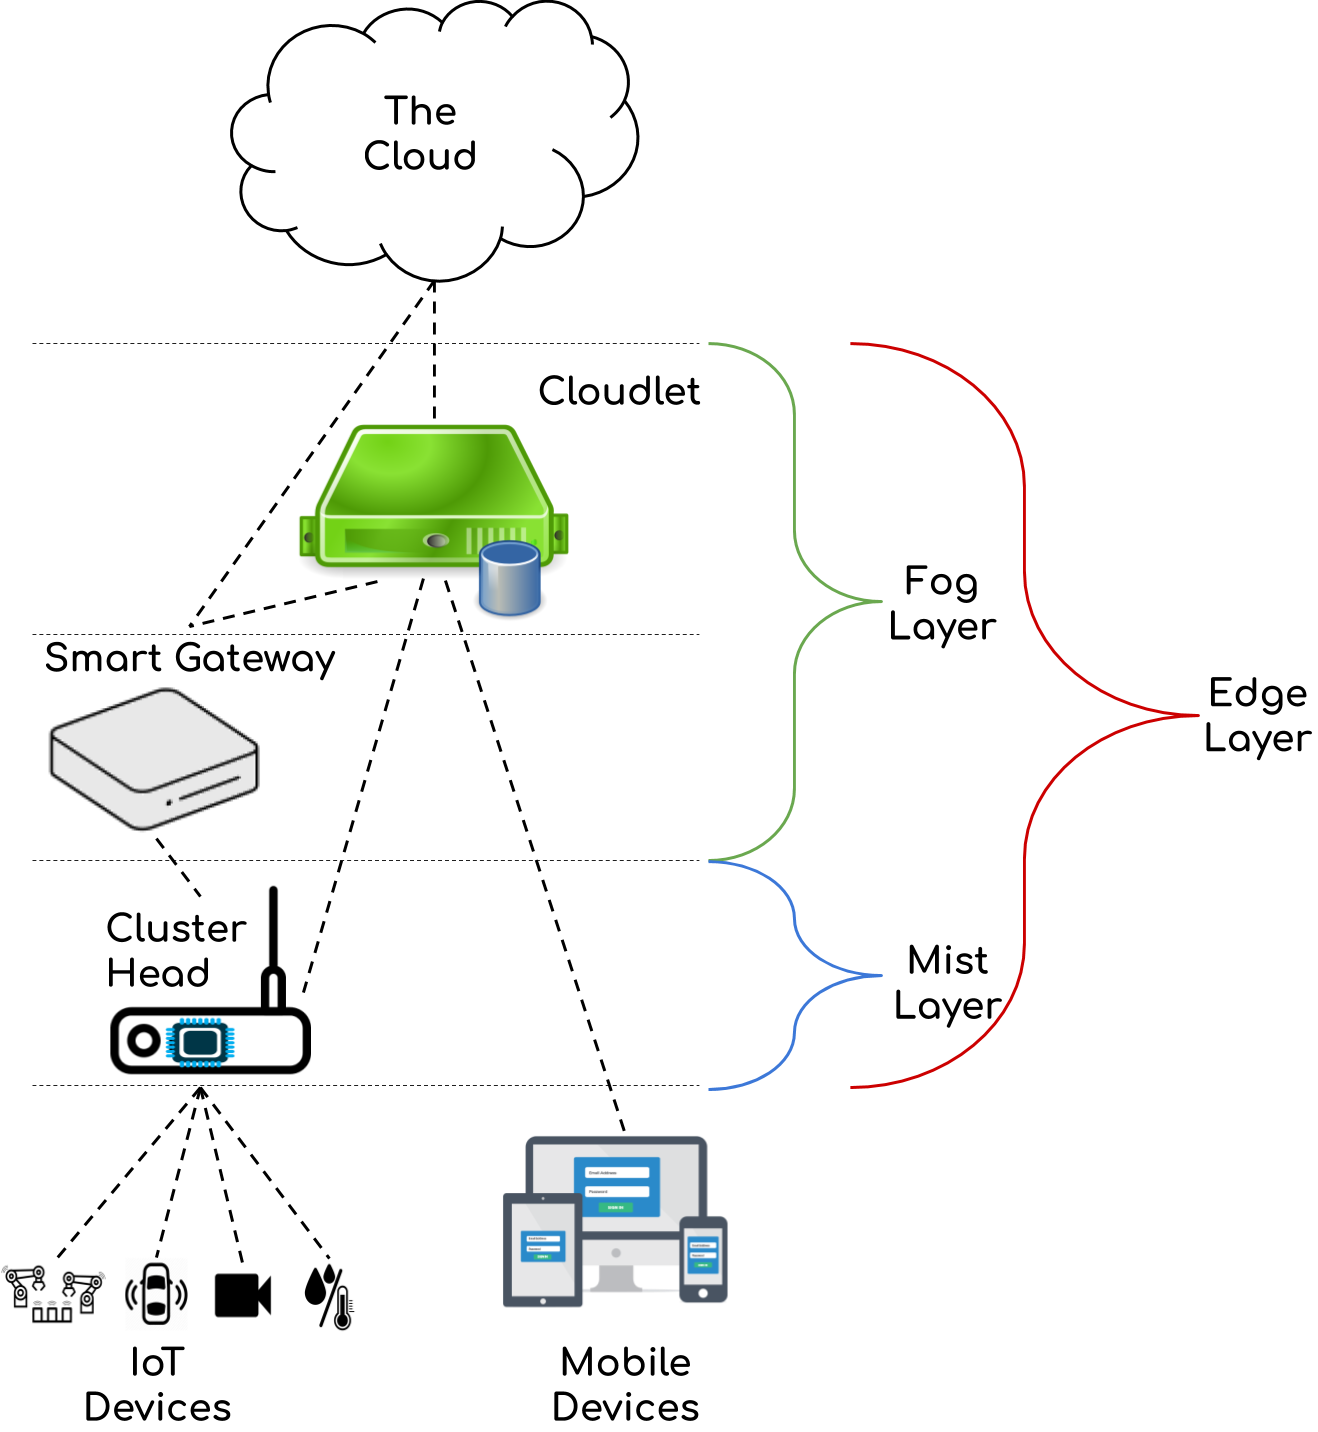
\includegraphics[scale=0.2]{figures/network-topology-3-layer.png}
    \caption{Three tier layer network topology, similar to \cite{nsa2017NextWaveIoTDef}}
    \label{fig:networkTopology3Layer}
\end{figure}

The cloud is well defined and understood. It describes the readily available computing resources over the Internet not managed by the user. The other layers and devices are not so well understood and defined separately.
\textbf{\textit{Constrained Device}}\\
Constraint devices are an elementary part of the IoT making up the "things"\cite{contstraintDevicesTerminology}.
They can have three main purposes. Either sensing or actuating (or both), where sensing is the 
passive action of measuring the environment (e.g. a motion detector) and actuating is the active action of influencing the environment (e.g. control of pressure in test tube). Or, finally, they can be smart objects enhancing the interaction between other smart objects and people.
They are usually defined by their limitation, mainly, small computing power (CPU, RAM, storage etc.) and limited power supply and operate in constrained network using protocols like BLE and ZigBee. \\[5mm]
\textbf{\textit{Smart/mobile devices}}\\
Smart devices are not clearly defined in the academic literature. I will use the definition given by \citeauthor{poslad2011smartDevices}\cite{poslad2011smartDevices}, to clearly divide them from constrained devices which this thesis will be concerned with. They are traditional computing devices and "tend to be multi purpose ICT devices"\cite{poslad2011smartDevices}, examples are mobile phones (smart phones) or tablets. They connect to the rest of the infrastructure directly but are free to move between networks. They also often rely on battery power and, importantly, are mainly end user devices. This has important privacy implication, a major factor for edge computing.\\[5mm]
\textbf{\textit{IoT Cluster Head}}\\
IoT Cluster Heads are defined by their very limited processing power. They are used to combine multiple sensors or actuators, but do not perform powerful operations. The line between IoT Cluster Heads and IoT Gateways is constantly moving as devices get more powerful and software more efficient. In this paper, IoT Cluster Heads are defined as devices which are used to read and control IoT devices but are not powerful enough to run containers or Kubernetes.
\textbf{\textit{IoT Gateway}}\\
IoT gateways are the connection between constrained devices and the cloud. I will use the term IoT gateway and not only gateway to stress its relation with IoT. They are usually connected to a network, either local or the the Internet. They facilitate inter-network and intra-network communications and because smart devices and especially constrained devices often communicate via wireless and non-Internet protocols, IoT gateways often translate protocols "between wireless sensor networks [...] and traditional communication networks"\cite{zhu2010iotGatewayDefinition}.
In recent years IoT Gateways have become a major field of interest and new research. As these devices got more powerful, developers started using them for pre-processing and data gathering locally at the edge.
IoT gateways can take a wide variety of forms. They can be simple L2/L3 routers or more powerful devices. Importantly, they are situated at the edge of a network.\\[5mm]
\textbf{\textit{Edge Layer}}\\
The edge layer is a term used to describe all resources sitting at the edge of the network. They do not interact with their environment directly only through IoT or mobile devices. This line started to fade, when mobile devices where used to control IoT devices directly. In this research I will stick to definition that edge layer devices are no user facing devices.\\[5mm]
\textbf{\textit{Fog Layer}}\\
The fog layer and consequently fog computing is a term used to describe the logical extension of traditionally cloud resources to the edge. These devices are still connected to the overall system and are an active part in the data processing pipeline. Fog computing enables repeatable structure on the edge for better and more scalable performance.
\textbf{\textit{Mist Layer}}\\
The mist layer is not logically connected to the cloud and both are not part of the same system and function independently of each other. It can be that the cloud can indirectly control the mist layer through the fog devices but importantly the mist layer does not do tasks which were traditional done in the cloud. \\[5mm]
\textbf{\textit{Edge cluster}}\\
Edge clusters are two or more edge devices working together where one device needs to be powerful enough to run a full control plane of the cluster technology. With emerging technologies like tiny builds of a full Kubernetes cluster, e.g. K3s from Rancher Labs\cite{k3sLight14:online}, this is becoming increasingly easier and more popular.
\footnote{Rancher provides a 40MB Kubernetes binary and claims that 500MB of RAM is sufficient 
it stable.}.\\
\textbf{\textit{Edge node}}\\
Edge nodes are defined as nodes "that act as an end user portal for communication with other
nodes in cluster computing"\cite{Whatised17:edgeNodeDef}. The other nodes can either be edge nodes as well or cloud nodes. Importantly, edge nodes do not need to be able to run their own control plane.
\subsection{Existing Solutions} \label{sec:existingSolutions}

Traditionally, edge devices were isolated cluster heads mainly forwarding traffic from their slaves to the cloud. Today, they are an integral part of the data flow pre-processing data and executing part of the business logic. But, there are still no coherent architectural as well as technological standards. In this section we will compare widely adopted and developed solutions in the industry to detect similarities and differences. The solutions also differ in age and 

% https://scholar.google.com/scholar?cluster=13680069378267225814&hl=de&as_sdt=0,5
% https://www.pac-online.com/sites/pac-online.com/files/upload_path/PDFs/Thema_des_Monats_Juni_2017_IoT_Plattformen.pdf
% https://blog.bosch-si.com/bosch-iot-suite/lessons-learned-using-kubernetes-in-iot-deployments/

\subsubsection{Bosch IoT Gateway Solutions}
\comment{https://www.bosch-iot-suite.com/service/gateway-software/}
The Bosch IoT Gateway Software\cite{BoschIoT13:online} is the "oldest" software analyzed. It is based on the OSGi technology\cite{osgiDefintion25:online}, which is an aliance driven project from the Open Services Gateway initiative (OSGi). It defines a set of specifications (with reference implemetation and tests) for a dynamic modular system based on so called bundles, third party software, running on the Java Virtual Machine (JVM)\footnote{This means it is possible to use other languages apart from Java which can run in a JVM, e.g. Kotlin.}. It is important to note that Bosch also supplies a cloud part which is based on Kubernetes.\\
The OSGi framework consists of a layered model shown in \cref{fig:osgiLayerModel}. 
\begin{figure}[h!]
    \centering
    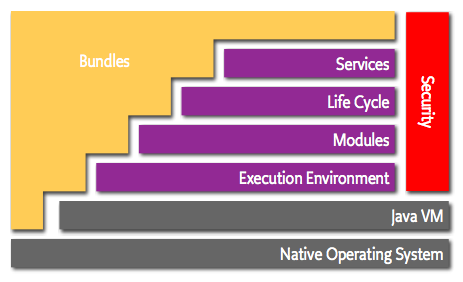
\includegraphics[scale=0.8]{figures/layering-osgi.png}
    \caption{From the official OSGI documentation\cite{osgiFrameworkArchitec22:online}.}
    \label{fig:osgiLayerModel}
\end{figure}
The Service layer interconnects the bundles making it possible for them to communicate via plain old java objects (POJO).The Life-Cycle layer handles the the state of the application (start, stop, update and uninstall). The Modules layer defines how an application can import and export code and the Execution Environemnt defines which methods and classes are available in a specific environemnt. Finally, the Security layer encompasses all other layers and handles for example code authentication, the digital signing of jar files, file access restrictions, certificates and more.\\
To the authors best knowledge there are currently five frameworks implementing the OSGi model besides the Bosch IoT Gateway Software\cite{BoschIoT13:online}. In a blog entry from 2015 Bosch compares the OSGi technology to other gateway solutions and says it "is the only one with clearly defined specs and an open specification process behind them"\cite{boschBlogOSGi69:online}. Boschs solution is proprietary and tailor made for edge-computing devices with IIoT in mind\cite{OSGiforIoTBlog27:online}. It runs on Linux, Windows, mac OS, Android, and VxWorks and according to Bosch more than 40 different gateway devices\cite{BoschIoT13:online}. The software is stable at major version 9 and still under heavy development. It is presented as exemplary software by the OSGi Alliance for IoT Gateways \cite{exampleIoTGateweOSGi:online} and thus used in this report. \Cref{fig:boschIoTGatewaySetup} shows where Boschs IoT solution is situated in the IoT environment. Bosch provides the OSGi framework implementation for the gateways and additional features for the cloud to ease the management of the gateways and store the accumulated data.
\begin{figure}[h!]
    \centering
    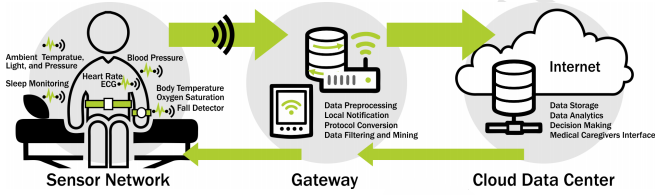
\includegraphics[scale=0.8]{figures/iotSetup.png}
    \caption{From the official Bosch documentation \cite{BoschIoT13:online}.}
    \label{fig:boschIoTGatewaySetup}
\end{figure}
Moreover, it supports a wide variety of communication protocls, BLE, ZigBee and MQTT, just to name a few. The main restriction is the JVM support for a protocol.  

\subsubsection{ioFog}
ioFog is one of the older projects in this report, with the first official release in 2016\cite{ioFogMainBlog:online}. Similarly to the OSGi framework it provides a runtime environment for applications, mainly intended for microservices. In addition, it includes a message bus, dynamic configuration of the microservices, and remote debugging\cite{ioFogMainBlog:online}. It runs on (almost) all Linux distributions and only requires Docker to be installed. In their official system requirements they only recommed using a Raspberry Pi as a worker node and not to run the Controller and Connector infrastructure \cite{ioFOgQuickStart:online}.
\Cref{fig:ioFogComponent} shows the fog computing layers in more detail.
\begin{figure}[h!]
    \centering
    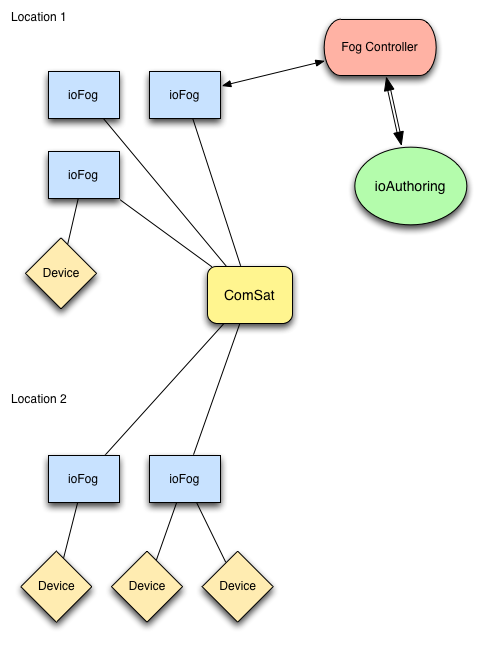
\includegraphics[scale=0.4]{figures/ioFog-Component_Diagram.png}
    \caption{hallo}
    \label{fig:ioFogComponent}
\end{figure}\\
The ioAuthoring application and the ioFog instances provide orchestration and management of the microservices. They are the main interaction points between the administrator and the system.
The fog computing software agent, called "ioFog", runs on various operating systems and provides a universal runtime for the IoT microservices. It includes a Software Development Kits (SDKs) in multiple programming languages to provide developers with the convenience of programming against standardized objects. The communication between different ioFog instances is facilitated through an internetworking utility that runs on popular Linux distributions, called "ComSat". Finally, for testing a tool for mimicking the fog computing runtime is included as well.\\
In a recent blog post from Mike Milinkovich, the Executive Director of the Eclipse Foundation Inc., he announced the initial availability of ioFog features that make any Kubernetes distribution edge-aware. He continuous saying that "these native Kubernetes enhancements are in the process of being contributed to the Eclipse ioFog open source project.", so not all features are available in the stable release as of the time of writing. But essentially, the ioFog Kubernetes APIs would provide standardized way of communication between the Kubernetes API Server and the ioFog instance.

\subsubsection{Docker Edge Solution}
Docker is commonly known for its containerization software and is often confused with the containers themselves (like google for search). The core container runtime, containerd, was donated by Docker to the Cloud Native Computing Foundry (CNCF) in 2017\cite{containerDonationDocker79:online} which manages and develops it now. Now, the company Docker focuses on providing an ecosystem around containers making them easy to deploy, secure and replicate. Recently, Docker announced a new partnerships with ARM and  a new strategy for edge devices.\\
\Cref{fig:dockerEdge} shows the Docker Edge Solution in context. 
\begin{figure}[h!]
    \centering
    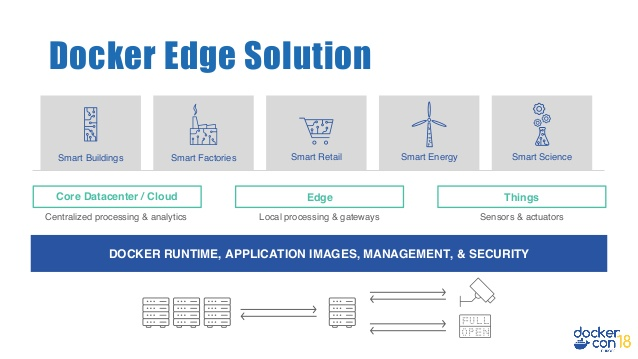
\includegraphics[scale=0.65]{figures/docker-edge-solution.jpg}
    \caption{Docker Edge solution .}
    \label{fig:dockerEdge}
\end{figure}
The solution consists of a few different products from its enterprise solution focusing on security, scalability/deployability and easy of use. The components are the same, but the edge focus is on fault tolerance and platform support, hence the new partnership with ARM. A core component of the suit is the docker registry, which can be mirrored/replicated on many difference servers for scaleability and fault tolerance. The edge registry can function without constant communication with the rest of the swarm. In case of no connection, the registry will only pull images which it already posses. As edge devices often have limitted disk space, docker only synchronizes promoted images on these nodes. Similarly to tags in git, promoted images are signed images that are explicitly marked as production ready. \cref{fig:dockerRegistryForIoT} shows registry management in the cloud (on the left) vs. on the edge (on the right).
\begin{figure}[h!]
    \centering
    \noindent\makebox[\textwidth]{
    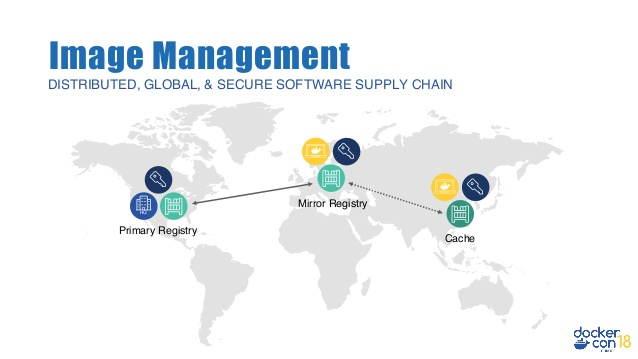
\includegraphics[width=(\textwidth+4cm)/2]{figures/docker-edge-computing-with-docker-enterprise.jpg}
    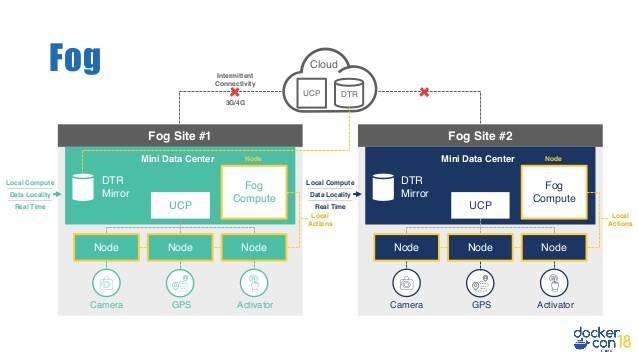
\includegraphics[width=(\textwidth+4cm)/2]{figures/docker-edge-registry-mirror.jpg}}
    \caption{The Docker registry in the cloud (left) vs. on the edge (right).}
    \label{fig:dockerRegistryForIoT}
\end{figure}
Whereas the cloud registry is build high availability (HA/LB) of the nodes in the swarm with fault tolerance against other nodes being unavailable, the edge registry is designed to have fault tolerance on it's own Internet access. In case of no connection it works as a standalone component, but synchronizes itself when it has a connection.\\
Importantly, the Docker Edge Solution is not a standalone solution, but integrates into the Docker ecosystem enabling remote management.

\subsubsection{K3s}
K3s is a "lightweight" kubernetes\footnote{Kubernetes is also known as k8s, hence the name k3s.} fork developed by Rancher\cite{rancherMainPage:online}. Similarly to Kubernetes and containerd, k3s is an open source project under the official management of the CNCF. It is also part of the Kubernetes IoT Edge working group explicitly aiming at bringing kubernetes related technologies to the edge. K3s is also a Certified Kubernetes distribution, meaning it confirms with the Kubernetes API standards. One of its big selling points is the good support for ARM64 and ARMv7 (targeting the Raspberry Pi and other smaller/less powerful single board computers). The traditional Kubernetes development is focused around the x86\_64 architecture, with limitted, and often untested, support for ARM, especially ARMv7. The co-founders of Rancher and developers behind k3s actually state in a webinar that half their development effort went into ensuring that all features they wanted work seamlessly on ARM\cite{k3sTalk:online}.\\
On their k3s product page \url{https://k3s.io/} Rancher describes the fork as follows:
\begin{displayquote}
Easy to install. A binary of less than 40 MB. Only 512 MB of RAM required to run.
\end{displayquote}
So k3s is not only significantly smaller than the full fledged Kubernetes install, but also requires significantly less resources at run time. It achieves this by mainly slimming down Kubernetes only including what they deem important for the edge. Because of the huge popularity of Kubernetes, it needs to support legacy code, drivers etc. K3s is free to break compatibility with older versions and the developers can instead focus on slimming down the code base much as possible. The lead developer, Darren Shepherd, said:
\begin{displayquote}
\textit{"We took Kubernetes and ripped out every single feature we didn't want.\cite{k3sTalk:online}"}
\\[1pt]
\raggedleft{{\rm --- Darren Shepherd}}
\end{displayquote}
K3s also integrates all process required by Kubernete, the Kubernetes master, Kubelet and containerd under one system process which requires less memory in total. \\
Another important aspect of k3s is its purpose to run on single as well as multi-node clusters. This is in stark contrast to Kubernetes, which is intended to run inside a cluster and it's fault tolerance model is build around on a multi-node cluster structure. Running a single node cluster is possible, but requires the tainting of the master node and is describe as "cheap and easy, but is not production grade" in the official documentation\cite{singleNodeKubernetesNotProductionDocumenhtation:online}.

\subsubsection{Kubeedge}
Kubeedge is another project inside the Kubernetes IoT Edge working group and thus build with Kubernetes in mind. It is a relatively young project to extend native containerized application orchestration and device management to the Edge. It is based on two parts, the cloud and the edge and (mainly) developed by Huawei, which at the time of writing could be reason for future complications because of recent US sanctions against the company.\\
The kubeedge system is shown in \cref{fig:kubeedgeStruct}.
\begin{figure}[h!]
    \centering
    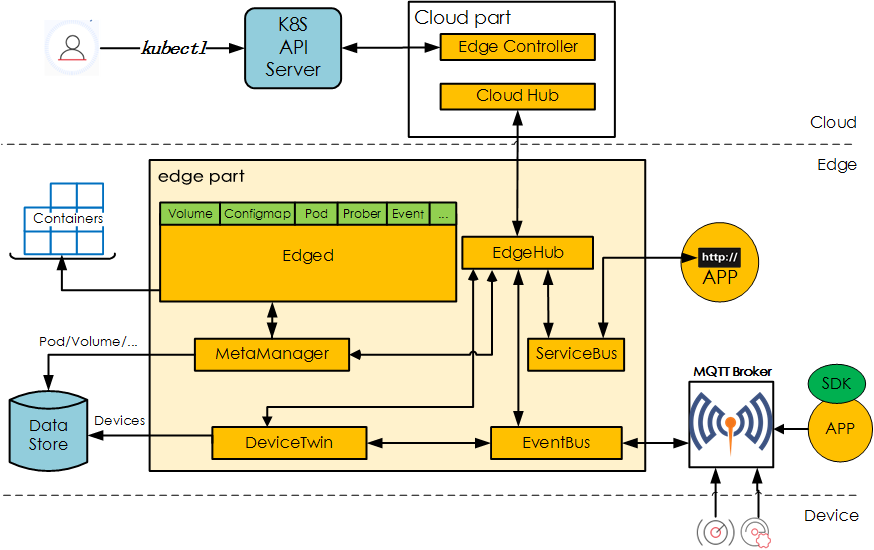
\includegraphics[width=(\textwidth+4cm)/2]{figures/kubeedge_arch.png}
    \caption{The Kubeedge system design.}
    \label{fig:kubeedgeStruct}
\end{figure}
The cloud part is built upon Kubernetes and provides support for application deployment, metadata synchronization and networking all through the Kubernetes API Server. The cloud and edge part communicate via web sockets. This means by design a good connection to the server is expected and the intend of the authors is to enable Fog computing. It is built upon Kubernetes and provides core infrastructure support for networking, application deployment and metadata synchronization between cloud and edge.\\
The edge part is not based on Kubernetes but uses similar concepts: Pods, volumes, events and more. It provides a life cycle management for containers and supports MQTT for communication for additional components. It also stores and synchronizes the device status to the cloud and has a query interface for local applications.

\subsubsection{Conclusion}
Only recently have industry behemoths like, Docker, Huawei, Bosch, Siemens, Red Hat, VMware and more\cite{K8sattheEdgeContectOnWorkingGroup:online} started to develop and, more importantly, concentrate their efforts on integrated IoT Gateway solutions. This lack of standardization is also acknowledged by the developers themselves ``While the problems at the IoT edge — connectivity, manageability, scalability, reliability, security — are being solved as point solutions by enterprises and ecosystem players, there is a need for a foundational industry-wide standard for managing distributed IoT workloads.''\cite{ioFogK8sBlog:online}\\
\Cref{tab:shortSotaSoftware} shows how the different solutions analyzed in this section compare to each other in key aspects.
% \footnote{An extended version can be found in the appendix.}
\begin{table}[h!]
% \hspace*{-2cm}
    \begin{center}
        
    \noindent\makebox[\textwidth]{
\resizebox{\columnwidth}{!}{%
\begin{tabular}{l|lll p{2.5cm} lllll}
                  & \begin{tabular}[c]{@{}l@{}}Open\\Source\end{tabular} & \begin{tabular}[c]{@{}l@{}}Centralized \\ control plane\end{tabular} & SW   &  Protocols  & \begin{tabular}[c]{@{}l@{}}System Req\\ control plane\end{tabular} & \begin{tabular}[c]{@{}l@{}}System Req\\ worker node\end{tabular} & \begin{tabular}[c]{@{}l@{}}Container\\based\end{tabular} & \begin{tabular}[c]{@{}l@{}}Kubernetes\\ in cloud\end{tabular} & \begin{tabular}[c]{@{}l@{}}Kubernetes\\ on edge\end{tabular} \\ \cline{1-10} 
Bosch IoT         & No                                                                                                                             & Yes (cloud)                                                                                                                                  & Java & ZigBee, Z-Wave, BLE and more        & Server grade                                                                                                                               & Edge grade                                                                                                                               & No                                                                                                                                & Some                                                                                                                                  & No                                                                                                                                   \\
ioFog             & Yes                                                                                                                            & Yes (cloud)                                                                                                                                  & Java & ZigBee, Z-Wave, BLE and more        & Server grade                                                                                                                               & Edge grade                                                                                                                               & Yes                                                                                                                               & Some                                                                                                                                  & No                                                                                                                                   \\
Docker\\Enterprise & No                                                                                                                             & Yes (cloud)                                                                                                                                  & Go   & ZigBee, Z-Wave, BLE and more        & Server grade                                                                                                                               & Edge grade                                                                                                                               & Yes                                                                                                                               & No                                                                                                                                    & No                                                                                                                                   \\
K3s               & Yes                                                                                                                            & Yes (both)                                                                                                                                   & Go   & Only IP based protocols             & Edge grade                                                                                                                                 & Edge grade                                                                                                                               & Yes                                                                                                                               & Yes                                                                                                                                   & Yes                                                                                                                                  \\
Kubeedge          & Yes                                                                                                                            & Yes (cloud)                                                                                                                                  & Go   & MQTT and IP. More planned & Server grade                                                                                                                               & Edge grade                                                                                                                               & Yes                                                                                                                               & Yes                                                                                                                                   & No                                                                                                                         
\end{tabular}}}
    \caption{Summary of the analyzed software.}
    \label{tab:shortSotaSoftware}
    \end{center}
\end{table}
It is important to bear in mind, that the Bosch IoT solution as well as ioFog are significantly older than the other projects. Boschs IoT solution is based on the OSGi framework. It provides isolation evolving around the JVM. This enables it to be platform independent, that is as long as the OS provides a JVM. ioFog which is almost three years old as of time of writing (June 2019) and already relays on containers, specifically a Docker runtime, for its deployment.\\
As the second last column shows all solutions, except for Docker Edge, use Kubernetes as their orchestration platform and control plane of choice. ioFog and Bosch IoT Edge are currently updating their solution while Kubeedge and K3s where designed from the ground up with Kubernetes in mind. However, only K3s tries to bring Kubernetes to the edge as well. This also means, that all solutions require different hardware requirements for the control plane, usually server grade hardware running containers, and more resource efficient solutions for the edge. \\
It is also important to note that all newer solutions, Docker Edge Solution\footnote{As the source code is not publicly available, this is speculative based on the fact that the main programming language for Docker is Go.} K3s and Kubeedge are developed in the Go programming language. Older systems are mainly based on Java as it enables code to run on every JVM supported platform. It is also important to note, that containers give developers freedom of programming language. The Bosch IoT Edge Solution and its use of the OSGi framework force developers into using a JVM compatible programming language. Docker points out that its solution runs on MacOS and Windows, however, both rely on Linux system calls.\footnote{Docker on Windows uses the WSL 2.0 in the future which translates Linux system calls to Windows system calls and increases performance a lot compared to emulated solutions as done on MacOS.}.\\
Another important aspect is protocol support. Here, the OSGi framework is clearly ahead as it has complete access to the system hardware, due to the JVM and also 



% From a design perspective, this is very similar to containers, where isolation is provided by Cspaces and Namespaces instead of process ID. Containers need access to communication 

% Giving access to devices like  Blt sigbee is a security issue.



\comment{
Should I include Azure IoT Edge as managed cloud iot gateway offering????\\

The problems at the IoT edge, connectivity, manageability, scalability, reliability, security, are being solved as point solutions by enterprises and ecosystem players, there is a need for a foundational industry-wide standard for managing distributed IoT workloads.


What is the purpose of this section?\\
problem area: what is actually the problem with the current system? hint into solution\\
competitor anaylsis: compare different approaches to solve the management and security of IoT gateways as well as solutions inside the individual categories. 


}
% \input{2.tex}
% \input{3.tex}
% \input{4.tex}
% \section{Argument which type of Knowledge Management and Enterprise Systems that may best suit the needs of the case organization (10\%)}
Agillic needs to cope with a wide variety of requirements for its Knowledge Management (KM) systems. The main forms of knowledge are tacit knowledge, project specific knowledge, organizational knowledge, company knowledge and external knowledge. \cite{jashapara2004knowledge} presents 5 different KM systems: Document management systems, decision support systems, group support systems, workflow support systems and customer relationship management systems.\\
For simplicity and considering the size of Agillic, there should be one big platform for providing extensive internal documentation. Jira \citep{jira} is a very popular documentation tool for agile project management and a good fit for Agillic. It can be used by the whole company without any modifications and supports different access right schemes for spaces (i.e. a sub-directory). To coordinate the workflow a simple email or chat tool, e.g. Slack \citep{slack} is enough.\\
The teams need to tackle various problems: how to get the right information to the right person at the right time, how to enhance the communication, knowledge sharing, cooperation, coordination, social encounters within groups and how to manage associated workflows \citep{jashapara2004knowledge}. Having a good documentation platform is enough for most organizations, however developers need an extra platform 
for version-control  (e.g. git) to share code and handle associated workflows via pull/merge requests. It is often a problem to keep documents updated between the version-control system and the documentation platform. Jira  has a plugin for gitlab and github, web based git managers, which do exactly that. They mirror the content between the two systems, so that the developer does not need to worry about updating both systems. Tacit knowledge is often not documented because the effort of doing so is greater than its benefits. So having an easy to use solution for taking notes inside the version-control system would be of great benefit. \\ 
Agillic should also introduce guidelines for good documentation including best practices on how to write and store documents. Similarly to opinionated software in the previous chapter, documentation guidelines reduce the documentation overhead. It eases the burden of the writer to find a good style and make it easier for other employees to find and read the documents. A good example for this is the morphological box in \cref{fig:kees} by \cite{kees2015characteristics} where the field for Agillics version-control system are highlighted. 
It represents a unified approach on how to classify enterprise systems on their maturity, target group, technology, dissemination and contracting. This would pave the way for new enterprise or KM systems to be introduced when the company outgrows the current one two system solution, while still maintaining a clear structure for all stakeholders.
\clearpage

\printbibliography[heading=bibintoc]
\clearpage

\let\svaddcontentsline\addcontentsline
\renewcommand\addcontentsline[3]{%
  \ifthenelse{\equal{#1}{lof}}{}%
  {\ifthenelse{\equal{#1}{lot}}{}{\svaddcontentsline{#1}{#2}{#3}}}}
 
 \pagenumbering{arabic}
 
% \begin{appendices}
% \section{Structural factors}
% \begin{figure}[ht]
%     \centering
   
%     \label{fig:cat_strcut_mintzberg}
%     \caption{Elements of the Five Structural Configuration by Mintzberg}
%      \includegraphics[scale=0.4]{pictures/mintzberg_table.png}\\
%      Source: \cite{mintzberg1980structure}
% \end{figure}

% \clearpage
% \section{Morphological Box for Agillics version-control system}
% \begin{figure}
%     \centering
%     \caption{Morphological box for enterprise software 5.0}
%     \includegraphics[scale=0.4]{pictures/kees.png}\\
%     Source: \cite{kees2015characteristics}
%     \label{fig:kees}
% \end{figure}


% \end{appendices}


\end{document}